%%%%%%%%%% Prefix a "S" to all equations, figures, tables and reset the counter %%%%%%%%%%
\setcounter{equation}{0}
\setcounter{figure}{0}
\setcounter{table}{0}
\setcounter{page}{1}
\makeatletter

\renewcommand{\theequation}{S\arabic{equation}}
\renewcommand{\thefigure}{S\arabic{figure}}
%%%%%%%%%%%%%%%%%%%%

\subsection{1D Map in the Immediate Relaxation Limit and its Derivative} \label{supp: sub1}
We seek a function $\phi_{i+1}(\phi_i, b, \tau)$ describing the system's dynamics in the limit $k \rightarrow \infty$. Using the law of cosines and noting $\angle{rb}= \pi-\phi 2\pi$ (see Fig. \ref{osc}), the radial coordinate $r'(r,\phi,b)$ after perturbation is:
\begin{align}
    r'&=\sqrt{r^2+b^2-2rb\cos(\pi-\phi 2\pi)}\\
     &=\sqrt{r^2+b^2+2rb\cos(\phi 2\pi)} 
     \label{eq: r}.
\end{align}
Again, using the law of cosines, the angular coordinate $\phi'(r,\phi,b)$ after perturbation is $r =\sqrt{r'^2+b^2-2r'b\cos(\phi' 2\pi)}$. Then 
\begin{align}
    \cos(\phi' 2\pi) &= \frac{r^2+b^2+2rb\cos(\phi 2\pi) +b^2 - r^2}{2r'b} \\
    &= \frac{b+r \cos(\phi 2\pi)}{\sqrt{r^2+b^2+2rb\cos(\phi 2\pi)}} \\
    \phi' &= \frac{1}{2\pi}\arccos(\frac{b+r \cos(\phi 2\pi)}{\sqrt{r^2+b^2+2rb\cos(\phi 2\pi)}})
\end{align} where Eq. \ref{eq: r} is used in lines S3 and S4. However, $\arccos(\cos(2\pi \phi')) = 2\pi \phi'$ only if $0\leq \phi' \leq 1/2$. This is because arccosine only inverts the first half-period of cosine function between $0$ to $\pi$. For $1/2 \leq \phi' \leq 1$, we note that $-\arccos(\cos(2\pi \phi')) +2\pi= 2\pi \phi'$. So over the complete range of possible perturbed phases, we have:
\begin{equation}
    \phi' =
    \begin{cases}
     \frac{1}{2\pi}\arccos(\frac{b+r \cos(\phi 2\pi)}{\sqrt{r^2+b^2+2rb\cos(\phi 2\pi)}}) & 0 \leq \phi' \leq 1/2 \\
    -\frac{1}{2\pi}\arccos(\frac{b+r \cos(\phi 2\pi)}{\sqrt{r^2+b^2+2rb\cos(\phi 2\pi)}}) + 1 & 1/2 \leq \phi' \leq 1 \\
    \end{cases}.
\end{equation}
Integrating the angular differential equation is trivial: $\phi_{i+1} = \textnormal{mod} \{\phi'_i + \tau,1\}$ (see equation \ref{eqn:2}), which adds $\tau$ to the above piecewise equation. 
\begin{equation}
    \phi_{i+1} =
    \begin{cases}
     \frac{1}{2\pi}\arccos(\frac{b+r \cos(\phi 2\pi)}{\sqrt{r^2+b^2+2rb\cos(\phi 2\pi)}}) + \tau & 0 \leq \phi' \leq 1/2 \\
    -\frac{1}{2\pi}\arccos(\frac{b+r \cos(\phi 2\pi)}{\sqrt{r^2+b^2+2rb\cos(\phi 2\pi)}}) + 1 +\tau & 1/2 \leq \phi' \leq 1 \\
    \end{cases}
    \label{eq: b_plot}
\end{equation}
Note that since the perturbations are horizontal, if $0 \leq \phi \leq 1/2$, then $0 \leq \phi' \leq 1/2$; and if $1/2 \leq \phi \leq 1$, then $1/2 \leq \phi' \leq 1$ (i.e. the perturbation never causes the system to cross the x-axis). For $b<1$, as $\tau$ is increased from 0, the phase response curve ($\phi_{i+1}(\phi_i)$) intersects the line $\phi_{i+1}= \phi_i$ tangentially (see Figure \ref{b_plot}). Hence, we conclude that for $b<1$, the type of bifurcation for the period-1 instability boundary is a tangent bifurcation. 

\indent It is useful to rewrite $\phi_{i+1}(\phi_i,b,\tau)$ in a different form, which makes it easier to calculate the derivative $\frac{\partial \phi_{i+1}}{\partial \phi_i}$. We begin by noting that $\arccos(x) = \cot^{-1}(\frac{x}{\sqrt{1-x^2}})$ for $|x|<1$ which is always satisfied for any $\phi$, $b$, $r$, if $x=\frac{b+r \cos(\phi_i 2\pi)}{\sqrt{r^2+b^2+2rb\cos(\phi_i 2\pi)}}$. Then, 
\begin{align}
    \frac{x}{\sqrt{1-x^2}} &= \frac{\frac{b+r_i \cos(\phi_i 2\pi)}{\sqrt{r_i^2+b^2+2r_i b\cos(\phi_i 2\pi)}}}{\sqrt{1-(\frac{b+r_i \cos(\phi_i 2\pi)}{\sqrt{r_i^2+b^2+2r_i b\cos(\phi_i 2\pi)}})^2}} & r_i = 1 \nonumber \\
    &= \frac{b + \cos(2\pi \phi_i)}{\sin(2\pi \phi_i)} \nonumber \\
    &= b\csc(2\pi \phi_i) + \cot(2\pi \phi_i)
\end{align} 
Which allows us to simplify the 1D map to,
\begin{equation}
    \phi_{i+1} =
\begin{cases}
        \frac{1}{2\pi}\cot^{-1}(b\csc(2\pi \phi_i)+\cot(2\pi \phi_i))+ \tau & 0 \leq \phi_i \leq 1/2 \\
       -\frac{1}{2\pi}\cot^{-1}(b\csc(2\pi \phi_i)+\cot(2\pi \phi_i))+ \tau + 1 & 1/2 \leq \phi_i \leq 1 \\
    \end{cases}.
\end{equation}
The derivative is calculated directly using the chain rule.
\begin{align}
    \phi_{i+1} &= \phi_i' + \tau \nonumber \\
    &= \frac{1}{2\pi}\cot^{-1}(b\csc(2\pi \phi_i)+\cot(2\pi \phi_i))+ \tau \nonumber \\
    \frac{\partial \phi_{i+1}}{\partial \phi_i} &= \frac{1}{2\pi} \frac{-\frac{\partial (b\csc(2\pi \phi_i)+\cot(2\pi \phi_i))}{\partial \phi_i}}{1+(b\csc(2\pi \phi_i)+\cot(2\pi \phi_i))^2} \nonumber \\
    &= \frac{1+b\cos(2\pi \phi_i)}{\sin^2(2\pi \phi_i)+\cos^2(2\pi \phi_i) + b^2 + 2b\cos(2\pi \phi_i)} \nonumber \\
    &=\frac{1+b\cos(2\pi \phi_i)}{1 + b^2 + 2b\cos(2\pi \phi_i)}
\end{align}

\subsection{Restrictions on $\tau$ for the period-1 instability boundary $b = \sqrt{4-3\sin^2(2\pi\tau)}$} \label{supp: sub2}

Next we check if there are any restrictions on $\tau$ for which $b = \sqrt{4-3\sin^2(2\pi\tau)}$ is not a period-1 instability boundary. Using the identity $\sin^2(2\pi\tau) + \cos^2(2\pi\tau) = 1$ and solving for $\tau$ we find:
\begin{align}
    b &= \sqrt{4-3(1-\cos^2(2\pi\tau))}\\
    \tau &= \frac{1}{2\pi}\arccos(\pm\sqrt{(b^2 - 1)/3}).
\end{align}
Since $\arccos(\cos(2\pi \tau)) = 2\pi \tau$ only if $0 \leq \tau \leq 1/2$ and $-\arccos(\cos(2\pi \tau)) +2\pi= 2\pi \tau$, for $1/2 \leq \tau \leq 1$, we can write:
\begin{equation} 
\tau =
\begin{cases}
        \frac{1}{2\pi}\arccos(\pm\sqrt{(b^2 - 1)/3}) & 0 \leq \tau \leq 1/2, 0 \leq \phi_i \leq 1/2 \\
       -\frac{1}{2\pi}\arccos(\pm\sqrt{(b^2 - 1)/3}) + 1 & 1/2 \leq \tau \leq 1, 1/2 \leq \phi_i \leq 1
    \end{cases}
\end{equation}
Note that $0 \leq \tau \leq 1/2$ implies $0 \leq \phi_i \leq 1/2$ for the period-1 cycle, which can be checked using $\tau = \phi_i - \phi'_i$ and $\phi'_i<\phi_i$. Similarly $1/2 \leq \tau \leq 1$ implies $1/2 \leq \phi \leq 1$ which can be checked using $\tau = 1-(\phi'_i - \phi_i)$ and $\phi'_i>\phi_i$.\\

\noindent Combing this result with the phase response curve $\phi_{i+1}(\phi_i)$, we get:
\begin{equation} \phi_{i+1} =
\begin{cases}
        \frac{1}{2\pi}\arccos(\frac{b+\cos(\phi_i 2\pi)}{\sqrt{1+b^2+2b\cos(\phi_i 2\pi)}}) + \frac{1}{2\pi}\arccos(\pm\sqrt{(b^2 - 1)/3}) & 0 \leq \phi_i \leq 1/2 \\
       -\frac{1}{2\pi}\arccos(\frac{b+\cos(\phi_i 2\pi)}{\sqrt{1+b^2+2b\cos(\phi_i 2\pi)}}) -\frac{1}{2\pi}\arccos(\pm\sqrt{(b^2 - 1)/3}) + 2& 1/2 \leq \phi_i \leq 1. \\
    \end{cases}
\end{equation}
However, when $1\leq b$, the period-1 condition $\phi_{i+1} = \textnormal{mod} \{\phi'_i + \tau,1\}$ at the instability boundary $\frac{\partial \phi_{i+1}}{\partial \phi_i} = -1$, is satisfied only for Eq \ref{eq:satisf} and not for Eq \ref{eq:reject}.

\begin{equation} 
    \tau =
    \begin{cases}
        \frac{1}{2\pi}\arccos(-\sqrt{(b^2 - 1)/3}) & 0 \leq \phi_i \leq 1/2 \\
       -\frac{1}{2\pi}\arccos(-\sqrt{(b^2 - 1)/3}) + 1 & 1/2 \leq \phi_i \leq 1
    \end{cases}
    \label{eq:satisf}
\end{equation} 

\begin{equation} 
    \tau =
    \begin{cases}
        \frac{1}{2\pi}\arccos(+\sqrt{(b^2 - 1)/3}) & 0 \leq \phi_i \leq 1/2 \\
       -\frac{1}{2\pi}\arccos(+\sqrt{(b^2 - 1)/3}) + 1 & 1/2 \leq \phi_i \leq 1
    \end{cases}
    \label{eq:reject}
\end{equation} 

At the $\frac{\partial \phi_{i+1}}{\partial \phi_i} = -1$ instability boundary, the phase must be a solution of $0 = 2+3b\cos(2\pi \phi_i) + b^2$:

\begin{equation} 
    0 = 
    \begin{cases}
       \phi_i - \textnormal{mod} \{\frac{1}{2\pi}\arccos(\frac{b+\cos(\phi_i 2\pi)}{\sqrt{1+b^2+2b\cos(\phi_i 2\pi)}}) + \frac{1}{2\pi}\arccos(-\sqrt{(b^2 - 1)/3}),1\}& 0 \leq \phi_i \leq 1/2 \\
       \phi_i - \textnormal{mod} \{-\frac{1}{2\pi}\arccos(\frac{b+\cos(\phi_i 2\pi)}{\sqrt{1+b^2+2b\cos(\phi_i 2\pi)}})-\frac{1}{2\pi}\arccos(-\sqrt{(b^2 - 1)/3}) + 2,1\}& 1/2 \leq \phi_i \leq 1 \\
    \end{cases}
    \label{eq:right}
\end{equation} 

\begin{equation} 
    0 = 
    \begin{cases}
       \phi_i - \textnormal{mod} \{\frac{1}{2\pi}\arccos(\frac{b+\cos(\phi_i 2\pi)}{\sqrt{1+b^2+2b\cos(\phi_i 2\pi)}}) + \frac{1}{2\pi}\arccos(+\sqrt{(b^2 - 1)/3}),1\}& 0 \leq \phi_i \leq 1/2 \\
       \phi_i - \textnormal{mod} \{-\frac{1}{2\pi}\arccos(\frac{b+\cos(\phi_i 2\pi)}{\sqrt{1+b^2+2b\cos(\phi_i 2\pi)}})-\frac{1}{2\pi}\arccos(+\sqrt{(b^2 - 1)/3}) + 2,1\}& 1/2 \leq \phi_i \leq 1 \\
    \end{cases}
    \label{eq:wrong}
\end{equation} 
The equation \ref{eq:right} is satisfied at the $\phi_i$ equal to the $\phi_i$ solutions of $0 = 2+3b\cos(2\pi \phi_i) + b^2$ while the equation \ref{eq:wrong} is satisfied for other $\phi_i$ values of the $\frac{\partial \phi_{i+1}}{\partial \phi_i} = -1$ instability boundary (see Fig \ref{instabbound} and Fig \ref{instabbound_restric}). Therefore, we reject Eq.(\ref{eq:reject}) as a solution to $\cos^2(2\pi\tau) = (b^2 - 1)/3$, which means $\cos(2\pi\tau) = -\sqrt{(b^2 - 1)/3}$ effectively restricts the period-1 instability boundary $b = \sqrt{4-3\sin^2(2\pi\tau)}$ to $1/4<\tau<3/4$, (see Fig \ref{p1-instab}). 

\section{Supplementary Figures}
\begin{figure}[H]
    \begin{center}
    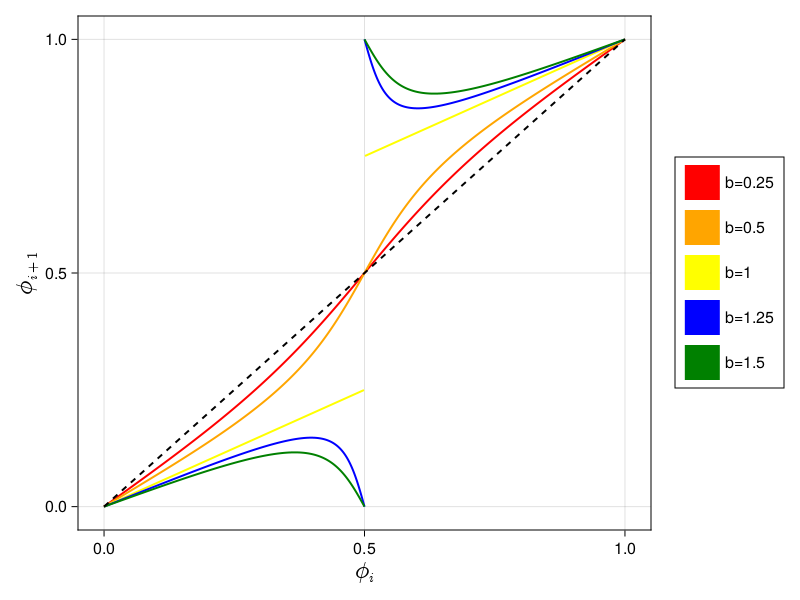
\includegraphics[width=.7\textwidth]{../plots/b_plot.png}
    \end{center}
\caption{Phase response curves $\phi_{i+1}(\phi_i)$, Eq. \ref{eq: b_plot}, for $k\rightarrow \infty$ and $\tau = 0$. The dashed line is the period-1 line where $\phi_{i+1}=\phi_i$.}
\label{b_plot}
\end{figure}

\begin{figure}[H]
    \begin{center}
    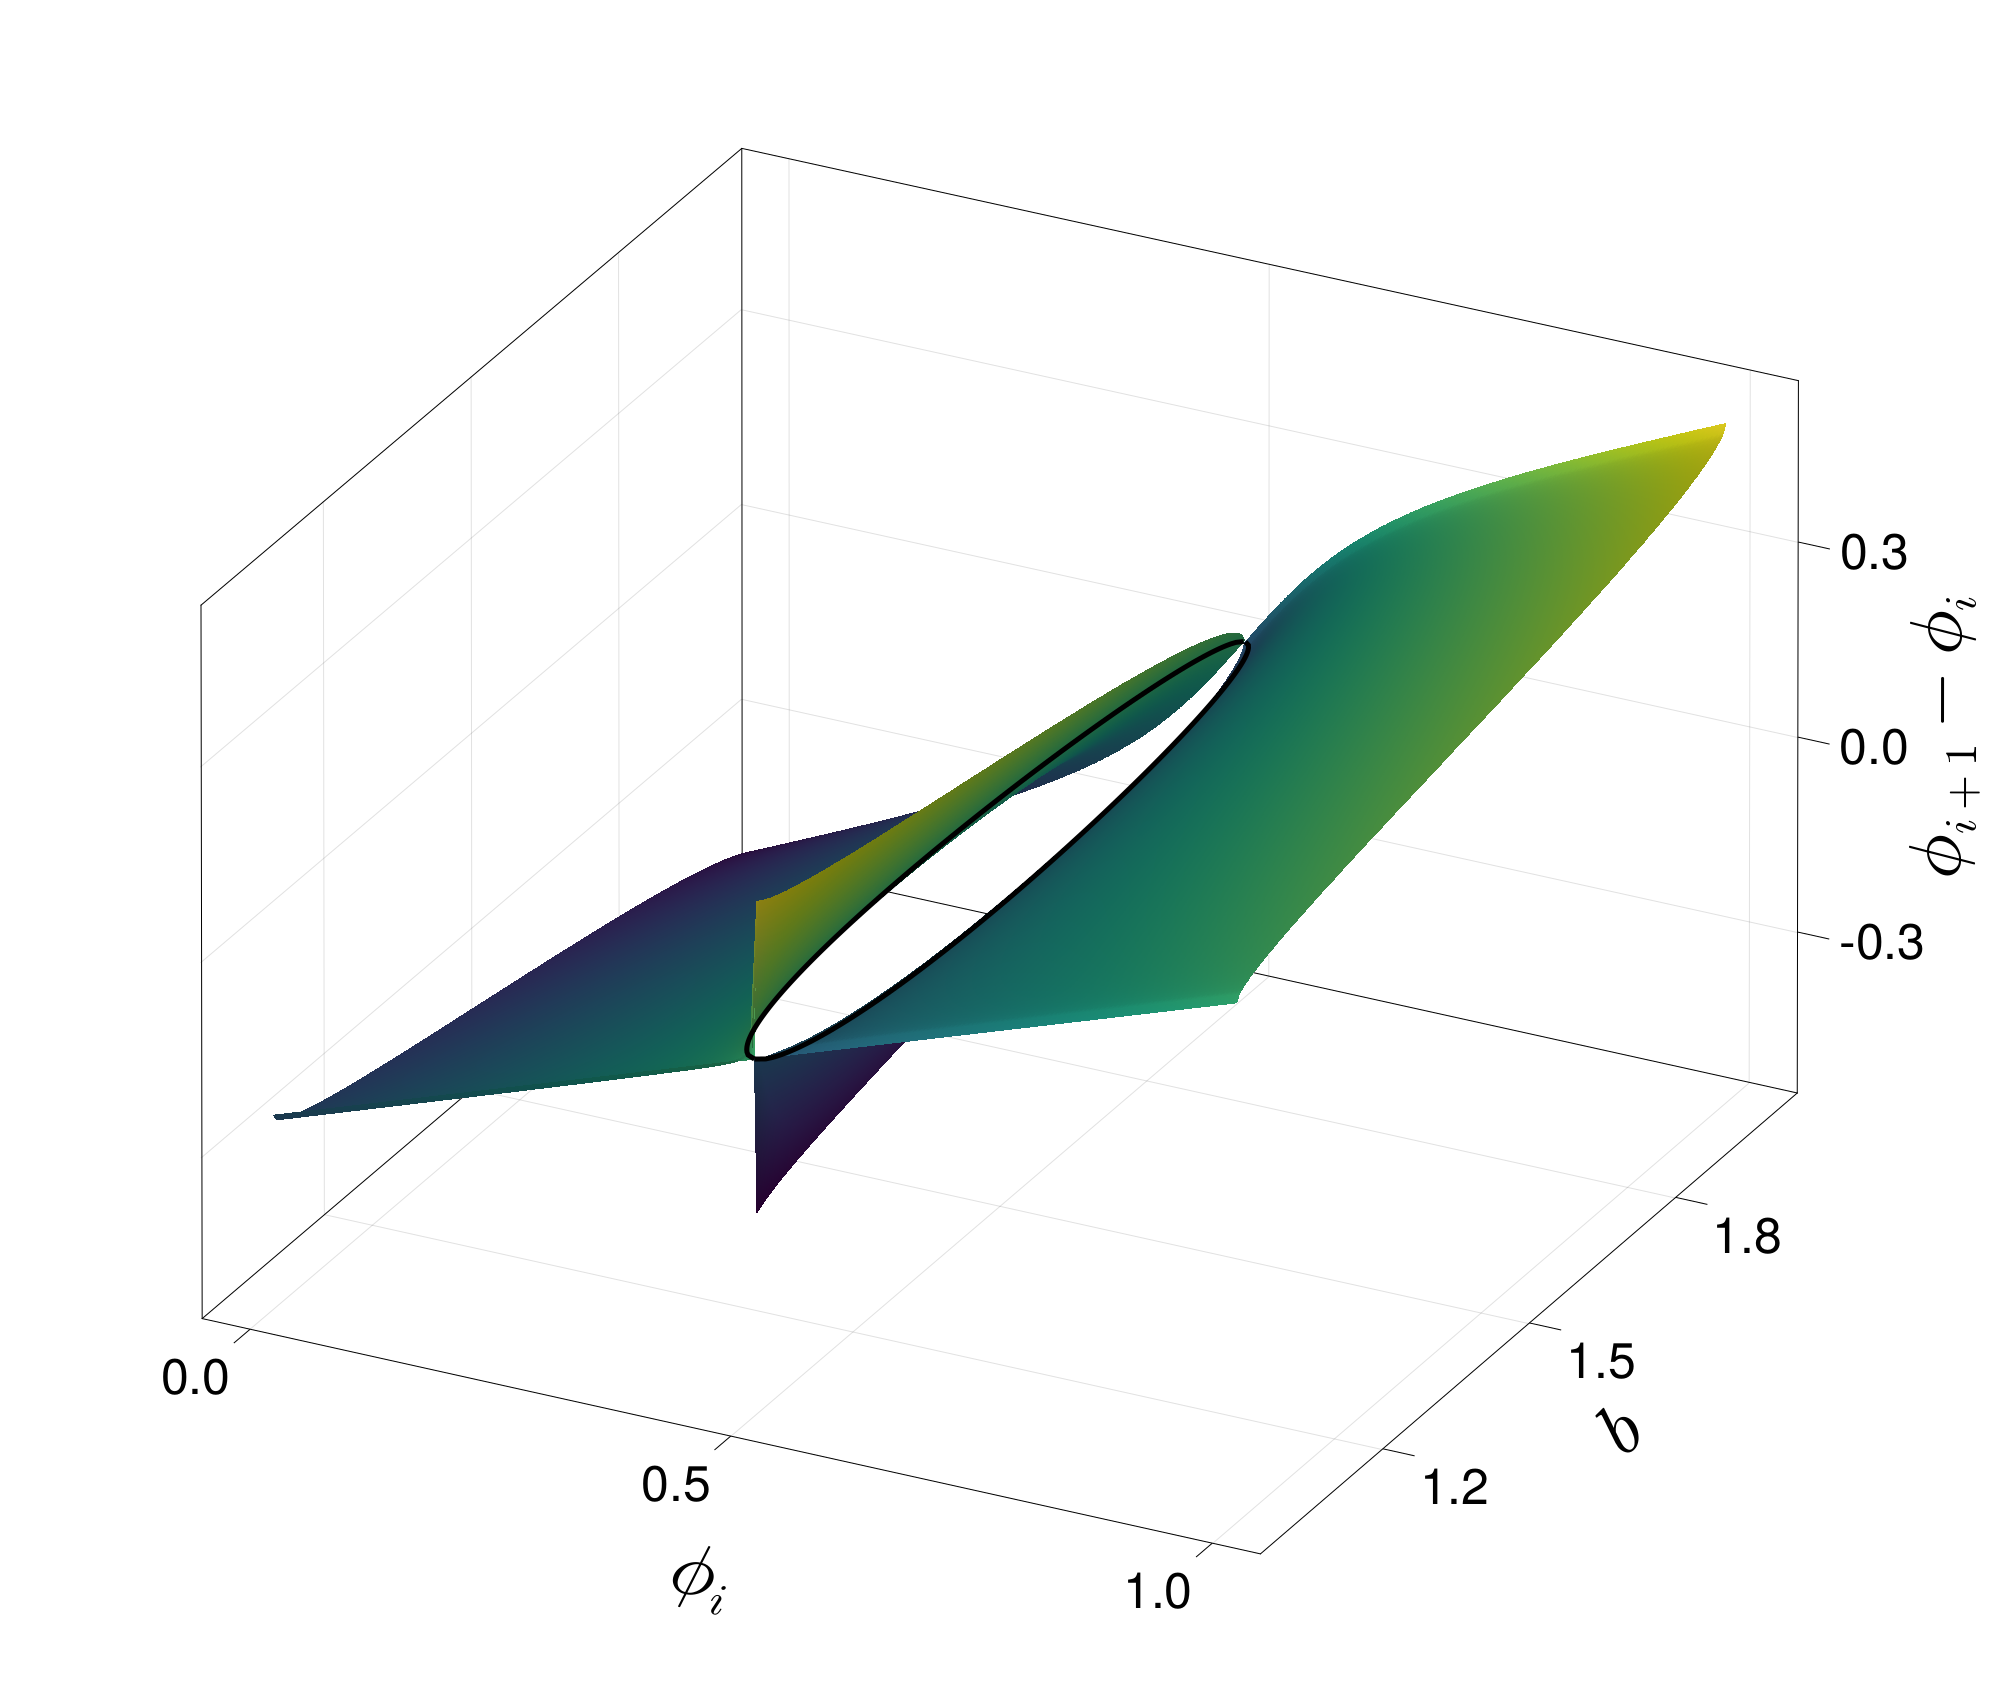
\includegraphics[width=.7\textwidth]{../plots/eqs17_fig.png}
    \end{center}
\caption{The above surface is Eq.(\ref{eq:right}). The black line is Eq.(\ref{eq:square}) where $\phi_{i+1}=\phi_i$. Eq.(\ref{eq:right}) fully intersects Eq.(\ref{eq:square}) where the period-1 condition ($\phi_{i+1}=\phi_i$) is satisfied.}
\label{instabbound}
\end{figure}

\begin{figure}[H]
    \begin{center}
    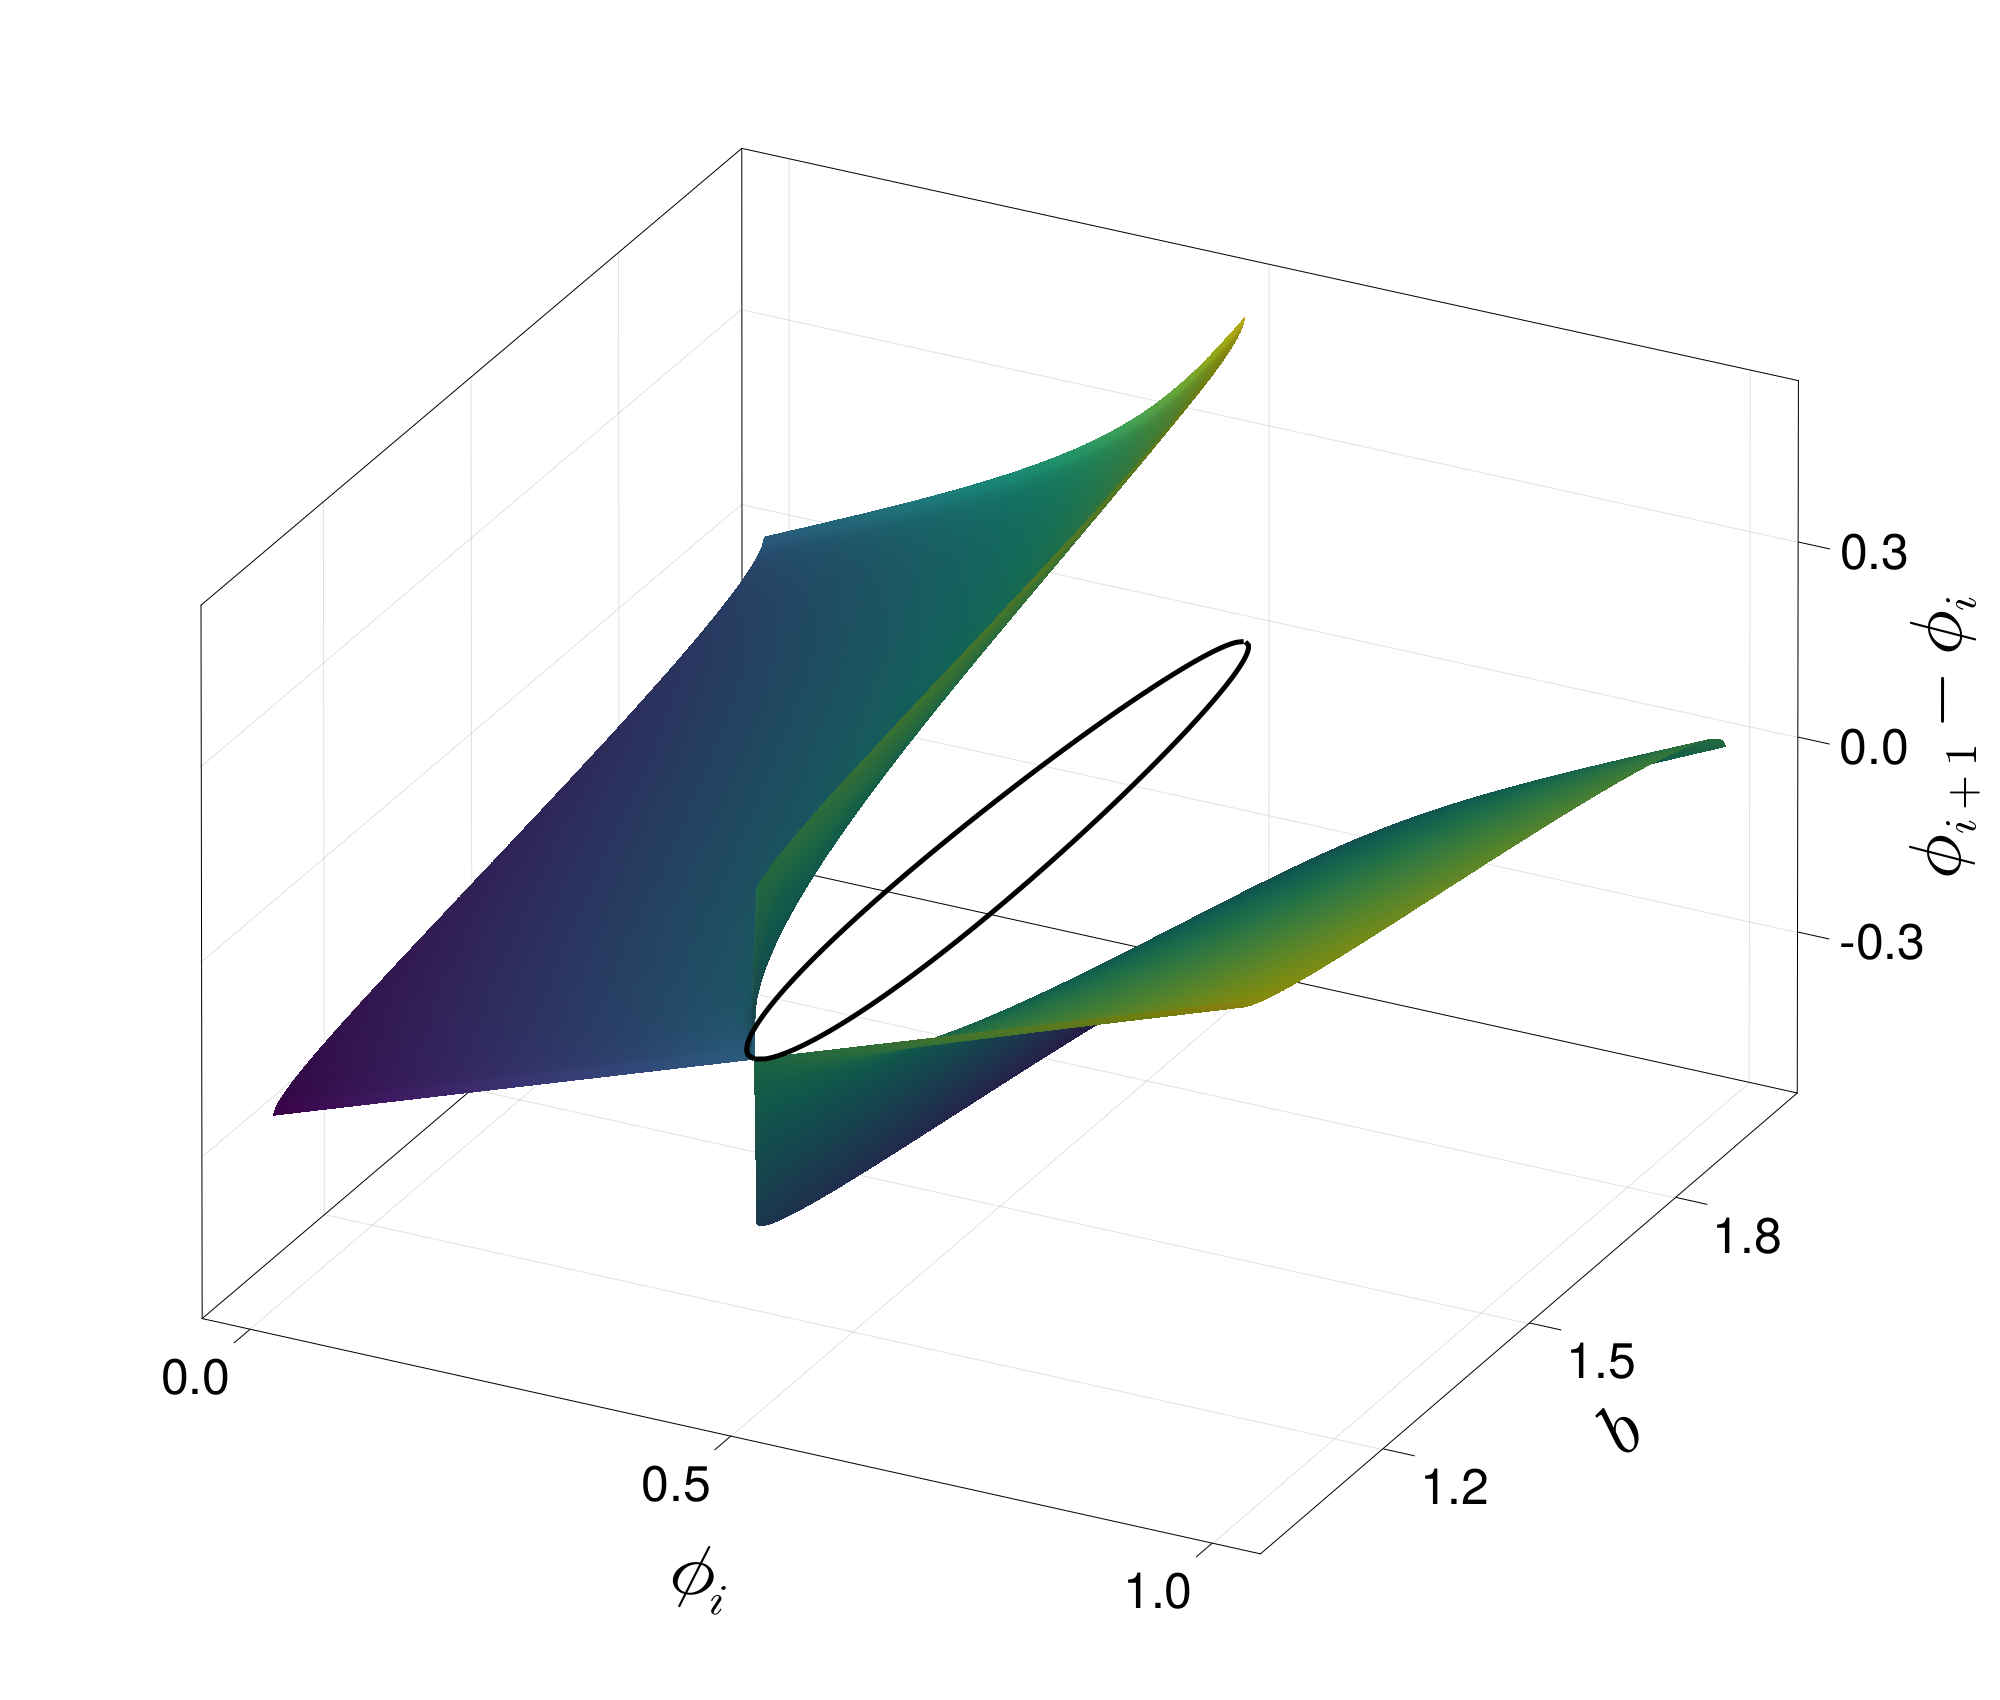
\includegraphics[width=.7\textwidth]{../plots/eqs18_fig.png}
    \end{center}
    \caption{The above surface is Eq.(\ref{eq:wrong}). The black line is Eq.(\ref{eq:square}) where $\phi_{i+1}=\phi_i$. Eq.(\ref{eq:wrong}) does not intersect Eq.(\ref{eq:square}) anywhere the period-1 condition ($\phi_{i+1}=\phi_i$) is satisfied.}
    \label{instabbound_restric}
\end{figure}

